\documentclass[12pt]{article}
\usepackage{epsfig}
\usepackage{cite}
\usepackage[bottom=0.88in, left=2cm, right=2cm]{geometry} % page margins


\usepackage{float}
\usepackage{siunitx}

\usepackage{xcolor}
\usepackage{colortbl}
\usepackage[utf8]{inputenc}
\usepackage[]{amsmath}
\usepackage{todonotes}
\usepackage{url}
\usepackage{verbatim}
\usepackage{pdfpages}
\usepackage{graphicx}% Include figure files
\usepackage{dcolumn}% Align table columns on decimal point
\usepackage{bm}
\usepackage{nccmath}
\usepackage{empheq}
\usepackage{hyperref}
\usepackage[utf8]{inputenc}
\usepackage{pdflscape}   
\usepackage{amsfonts}
\usepackage{listings}
\usepackage[newfloat]{minted}
\usepackage{caption}

%\usepackage{courier}
\usepackage{listings}

\marginparwidth 0pt
%\oddsidemargin  -0.6in
%\evensidemargin  0.0pt
\marginparsep 0pt
\topmargin   0pt
%\textwidth   7.5in
\textheight   8.5in 

\renewcommand{\baselinestretch}{1.0}

\def\bk{\bigskip}
\def\nd{\noindent}

\def\begdis{\begin{displaymath}}
\def\enddis{\end{displaymath}}
\def\begeq{\begin{equation}}
\def\endeq{\end{equation}}

\def\refs{{\bf \Blue{[Refs]}}}
\def\refsp{{\bf \Blue{[Refs] }}}


\def\begitem{\begin{itemize}}
\def\enditem{\end{itemize}}
\def\begdis{\begin{displaymath}}
\def\enddis{\end{displaymath}}
\def\begeq{\begin{equation}}
\def\endeq{\end{equation}}
\def\bk{\bigskip}       
\def\sk{\smallskip}
\def\mk{\medskip}
\def\nd{\noindent}

\definecolor{mintedbackground}{rgb}{0.95,0.95,0.95}

\newmintedfile[pythoncode]{py}{
bgcolor=mintedbackground,
%fontfamily=tt,
linenos=true,
numberblanklines=true,
numbersep=5pt,
gobble=0,
frame=leftline,
framerule=0.4pt,
framesep=2mm,
breaklines = true,
funcnamehighlighting=true,
tabsize=4,
obeytabs=false,
mathescape=false
samepage=false, %with this setting you can force the list to appear on the same page
showspaces=false,
showtabs =false,
texcl=false,
}

\newmintedfile[amplcode]{ampl}{
bgcolor=mintedbackground,
%fontfamily=tt,
linenos=true,
numberblanklines=true,
numbersep=5pt,
gobble=0,
frame=leftline,
framerule=0.4pt,
framesep=2mm,
breaklines = true,
funcnamehighlighting=true,
tabsize=4,
obeytabs=false,
mathescape=false
samepage=false, %with this setting you can force the list to appear on the same page
showspaces=false,
showtabs =false,
texcl=false,
}

\lstdefinelanguage{AMPL}{keywords={set,param,var,arc,integer,minimize,maximize,subject,to,node,sum,in,Current,complements,integer,solve_result_num,IN,contains,less,suffix,INOUT,default,logical,sum,Infinity,dimen,max,symbolic ,Initial,div,min,table,LOCAL,else,option,then,OUT,environ,setof ,union,all,exists,shell_exitcodeuntil,binary,forall,solve_exitcodewhile ,by,if,solve_messagewithin,check,in,solve_result
},sensitive=true,comment=[l]{\#}}

\lstset{frame=tb,
  language=AMPL,
  aboveskip=3mm,
  belowskip=3mm,
  showstringspaces=false,
  columns=flexible,
  basicstyle={\ttfamily},
  numbers=none,
  numberstyle=\tiny\color{gray},
  keywordstyle=\bfseries,
  commentstyle=\textit,
  stringstyle=\color{mauve},
  breaklines=true,
  breakatwhitespace=true,
  tabsize=3
}
\title{Network Level Sets - \( \lambda\)-\(\omega\) systems  (Protopaper)}
\author{}
\date{\today}

\newcommand{\hgr}[2][inline]{\todo[#1, color=blue!20!white]{\small \texttt{HGR}: #2}}
\newcommand{\cod}[2][inline]{\todo[#1, color=green!20!white]{\small \texttt{GVB}: #2}}
\setlength\parindent{0pt}

\newenvironment{code}{\captionsetup{type=listing}}{}
\SetupFloatingEnvironment{listing}{name=Listing}


\begin{document}

\begin{titlepage}

\begin{center}
\vspace*{-1in}
\begin{figure}[htb]
\begin{center}

\includegraphics[width=5cm]{logo_upc.jpeg}
\end{center}
\end{figure}

\begin{Large}
Models and Methods for Operation Research\\
\end{Large}
\vspace{4cm}
\vspace*{0.2in}
\begin{Huge}
\textbf{Solving The Traveling Salesman Problem (TSP)}\\
\end{Huge}
\vspace*{0.3in}
\begin{large}
Guillermo Villanueva Benito\\
\end{large}
\vspace*{0.3in}
\rule{80mm}{0.1mm}\\
\vspace*{0.1in}
\begin{large}
December 2021 \\
\end{large}
\end{center}

\end{titlepage}



%\maketitle
\newpage

\tableofcontents
\newpage

%\maketitle

\section{TSP data}
We are considering the solution of the symmetric version of the TSP over a complete graph $G=(V,E)$ with $n = |V|$ nodes. More specifically, our graph have 12 nodes, $n=12$. Moreover, since it is a complete graph the number of edges is
\begin{equation}
    |E| = \frac{n(n-1)}{2} = 66
\end{equation}
The graph is non-directed and each edge $(i,j)$ has its associated cost $c_{i,j}$ satisfying 
\begin{equation}
    c_{i,j} = c_{j,i}
\end{equation}
in order to compute the solution of the symmetric TSP.\\

We consider the following cost matrix $C$
\begin{equation}
    C = 
\resizebox{0.9\linewidth}{!}{$
        \left[ \begin {array}{cccccccccccc} 
        
         0.  &  0.723& 1.046& 0.811& 0.588& 0.547& 0.97&  0.452& 0.361& 0.444& 0.605& 0.359\\
         0.723 &0.   & 0.844 &0.618 &0.455 &0.186 &0.276 &0.534 &0.467 &0.306 &0.707& 0.39 \\
         1.046 &0.844 &0.    &0.255 &0.498 &0.791 &0.773 &0.597 &0.716 &0.954 &0.463 &0.975\\
         0.811 &0.618 &0.255 &0.    &0.244 &0.543 &0.609 &0.359 &0.468 &0.701 &0.288 &0.72 \\
         0.588 &0.455 &0.498 &0.244 &0.    &0.33  &0.551 &0.156 &0.231 &0.467 &0.255 &0.479\\
         0.547 &0.186 &0.791 &0.543 &0.33  &0.    &0.425 &0.369 &0.285 &0.185 &0.562 &0.248\\
         0.97  &0.276 &0.773 &0.609 &0.551 &0.425 &0.    &0.681 &0.661 &0.578 &0.798 &0.658\\
         0.452 &0.534 &0.597 &0.359 &0.156 &0.369 &0.681 &0.    &0.134 &0.448 &0.212 &0.431\\
         0.361 &0.467 &0.716 &0.468 &0.231 &0.285 &0.661 &0.134 &0.    &0.324 &0.344 &0.299\\
         0.444 &0.306 &0.954 &0.701 &0.467 &0.185 &0.578 &0.448 &0.324 &0.    &0.659 &0.088\\
         0.605 &0.707 &0.463 &0.288 &0.255 &0.562 &0.798 &0.212 &0.344 &0.659 &0.    &0.642\\
         0.359 &0.39  &0.975 &0.72  &0.479 &0.248 &0.658 &0.431 &0.299 &0.088 &0.642 &0.\\
        
        
        \end {array}
        \right]     
$}

\end{equation}
In order to compute cost matrix C, we have used a simple python code, Listing (\ref{ll1}). We have randomly generated 12 points in the region $[0,1]\times[0,1] \subset \mathbb{R}^{2}$ associated with the position of the 12 nodes of the graph. For each node $v_{i} \in V$ it position $p_{i}$ is 
\begin{equation}
    p_{i} = (x_{i},y_{i})
\end{equation}
Then, the cost matrix C is the distance matrix. More specifically, for each pair of nodes ($v_{i},v_{j}$) its associated cost $c_{i,j}$ is given by
\begin{equation}
    c_{i,j} = \|p_{i}-p_{j}\| = \sqrt{(x_{i} - x_{j})^{2} + (y_{i} - y_{j})^{2}}
\end{equation}

A graphical representation of this graph is shown in Figure (\ref{f1}).

\begin{figure}[H]
\centering
    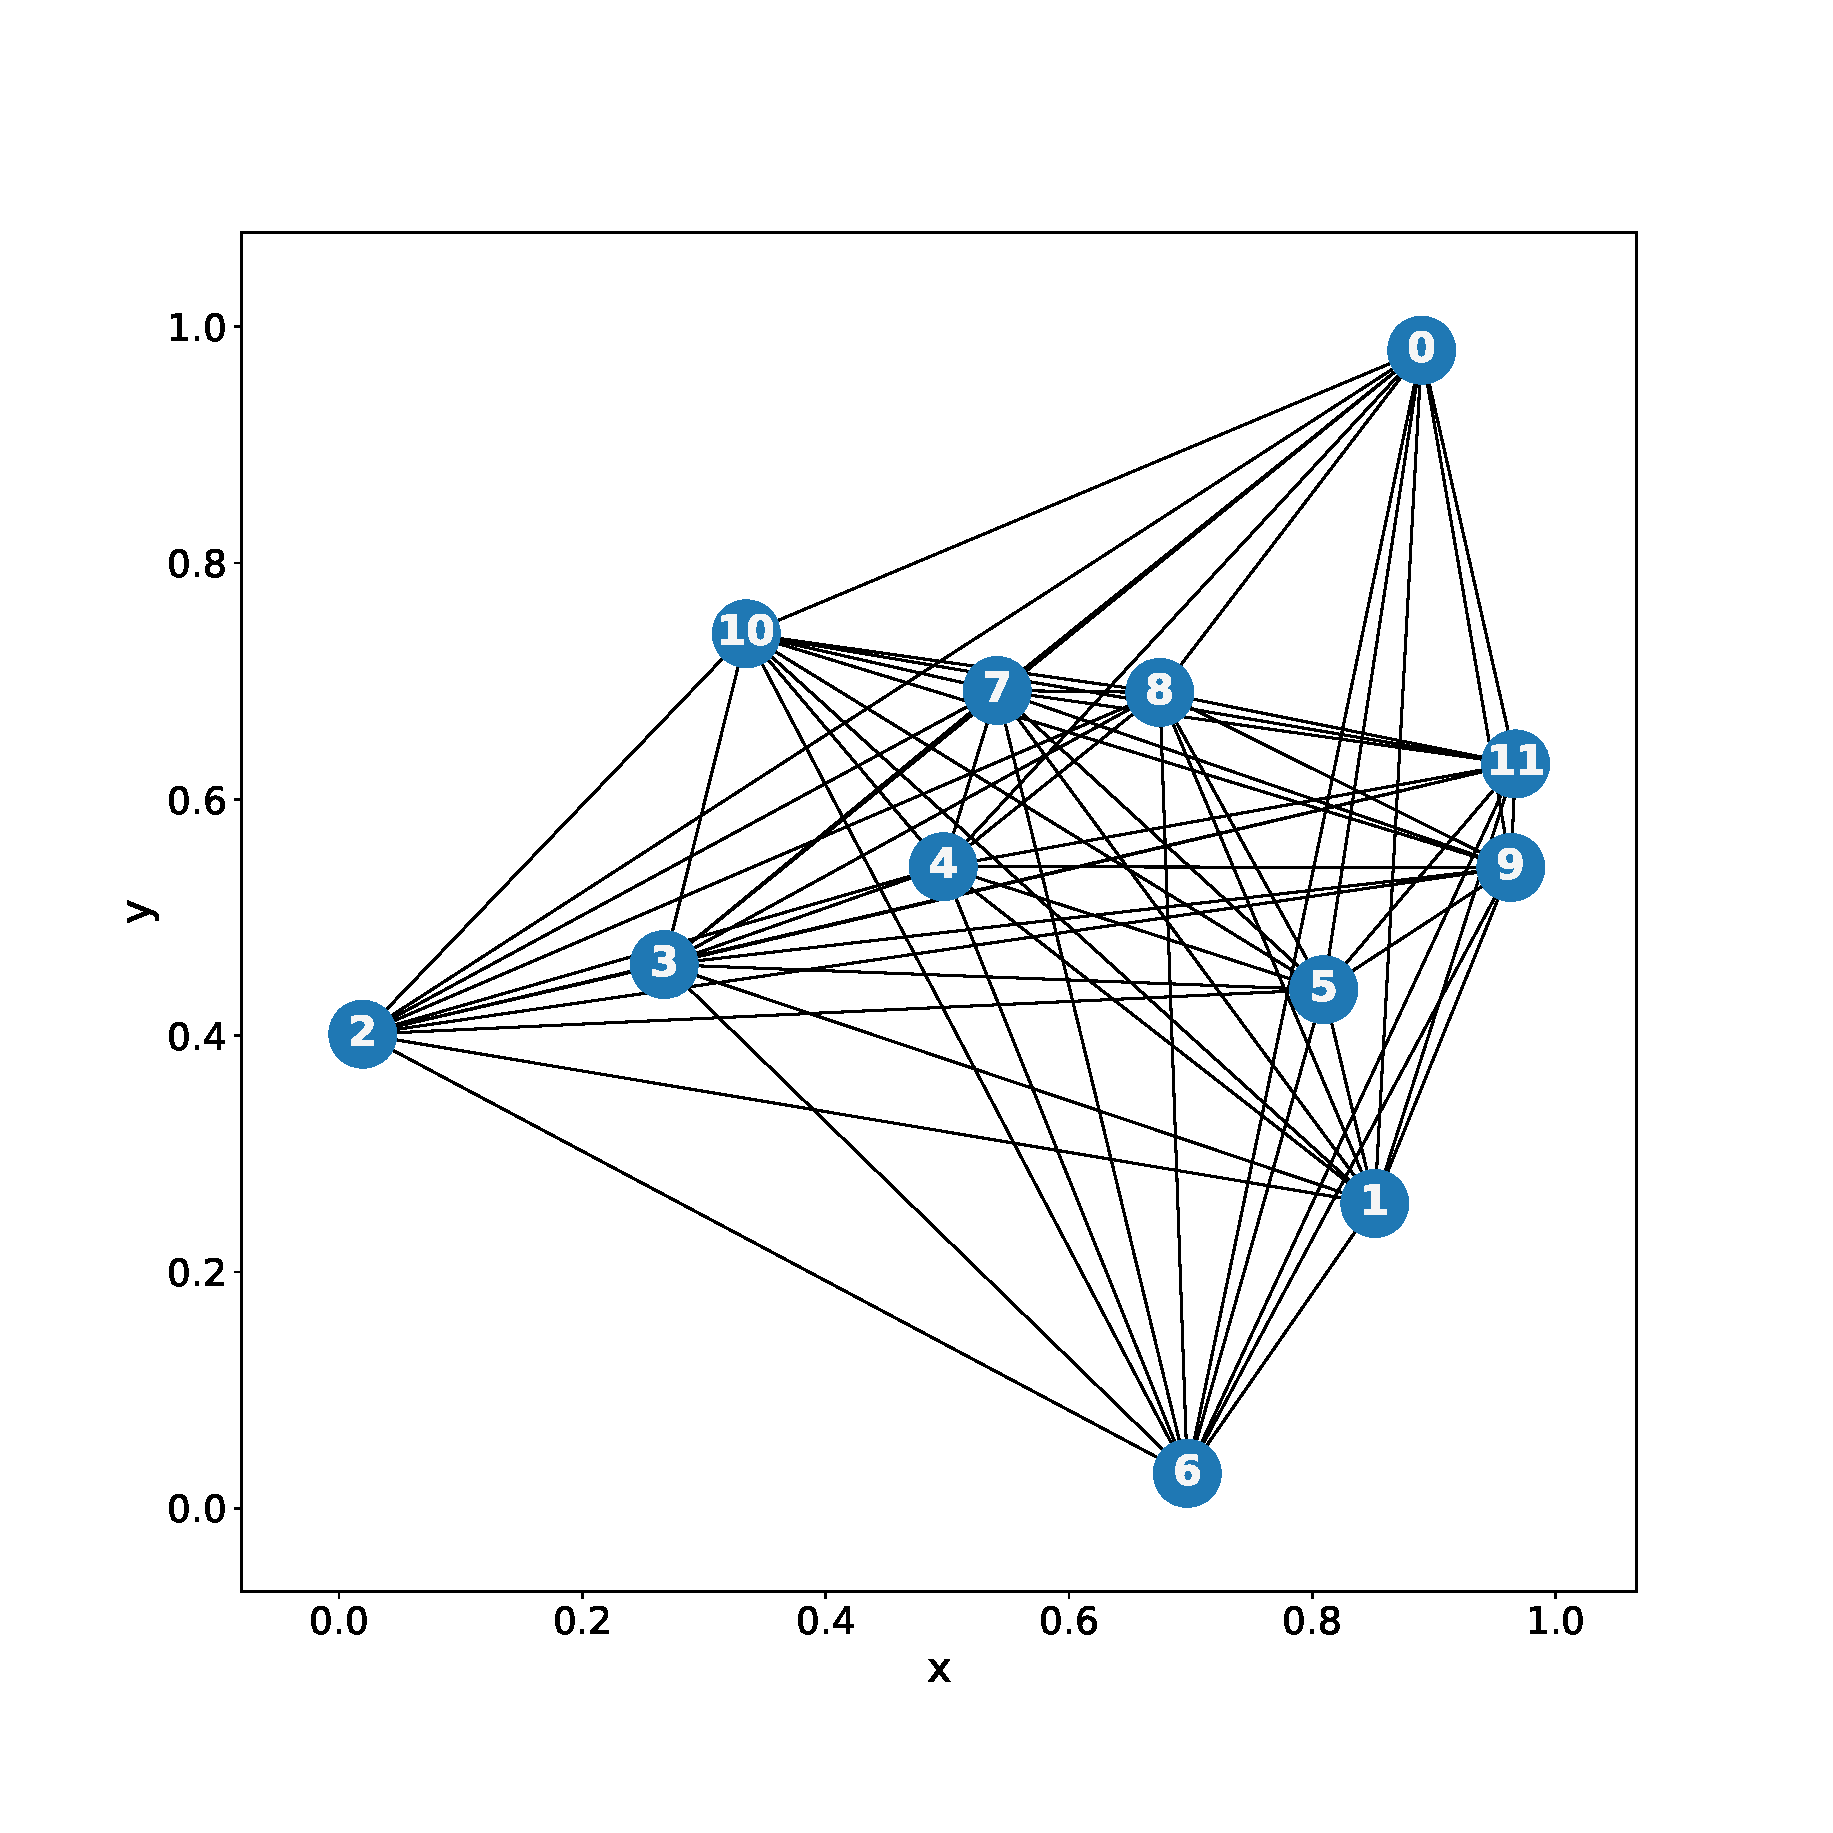
\includegraphics[width=1\linewidth]{1.eps} 
  \caption{Graph representation}
  \label{f1}
\end{figure}

\begin{code}
\captionof{listing}{Code section 1}
\label{ll1}
\pythoncode{1.py}
\end{code}


\section{Obtaining an upper bound}
In this section we program an heuristic for getting a feasible solution for the symmetric TSP (STSP). The heuristic will consist of two different parts: one constructive part, in which a greedy procedure is applied, and a second part, which consists of an improvement phase.\\

For the constructive part we will use the Nearest Neighbor primal heuristic.\\

\textbf{Nearest Neighbor (NN) heuristic:} Start at an arbitrary node $i_{1}$ and construct a path\\ $i_{1},i_{2},\dots,i_{j},i_{j+1},\dots,i_{n}$ where $i_{j+1} = \text{arg}(\text{min}(c_{i,k}: k \in V \backslash \{i_{1},i_{2},\dots,i_{j} \} ))$.\\

For the improvement phase, we will apply the 2-Interchange local search heuristic to obtain better upper bounds for the original TSP.\\

\textbf{2-Interchange local search heuristic:} Start with a given tour (feasible solution) and replace each pair of non-adjacent edges in the tour with the unique pair of replacement edges if the resulting tour has a lower weight.\\

The main results of this section are shown in Figure (\ref{f2}). Here, we have applied the 2-Interchange local search heuristic to 12 initial tours. Each tour is the output solution for the NN heuristic taking a different initial arbitrary node. For instance, the red curve (NN(3)) shows the different improving tours obtained by the 2-Interchange local search heuristic taking as initial tour, the tour solution for the NN heuristic with initial node, node number 3. The initial upper bound is the upper bound obtained using only the NN heuristic.

\begin{figure}[H]
\centering
    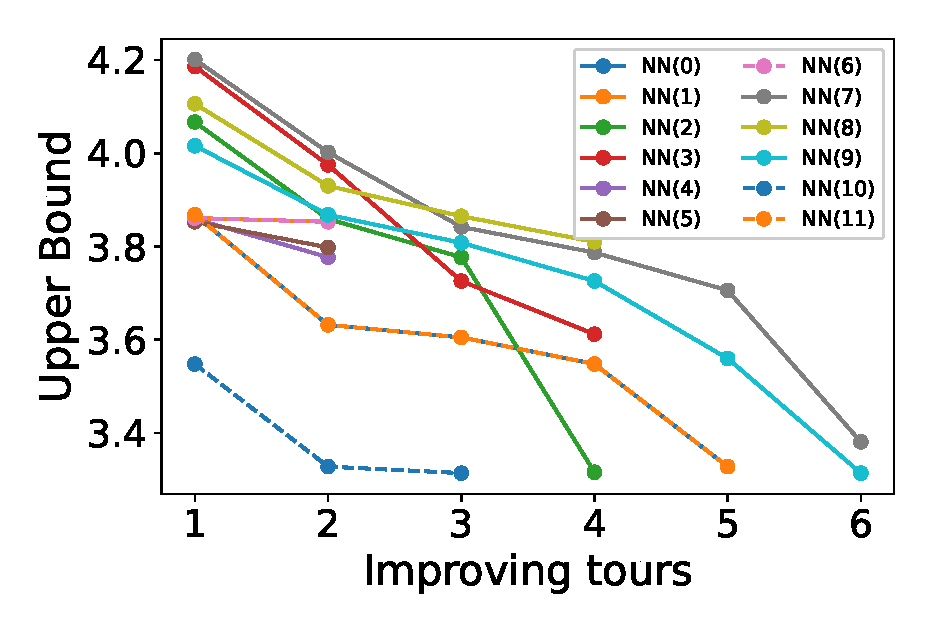
\includegraphics[width=0.6\linewidth]{10.eps} 
  \caption{Upper bounds as a function of the different improving tours obtained by the 2-Interchange heuristic. The first upper bound is the upper bound obtained using the NN heuristic with initial node given by the color legend.}
  \label{f2}
\end{figure}

As expected, the local search heuristic improves the upper bound obtained by the greedy heuristic. We notice that the best upper bound has been obtained with NN(9) and NN(10). In both cases, the obtained upper bound is

\begin{equation}
    \overline{z^{*}} = 3.314
\end{equation}

and the resulting tour is shown in Figure (\ref{f3}).

\begin{figure}[H]
\centering
    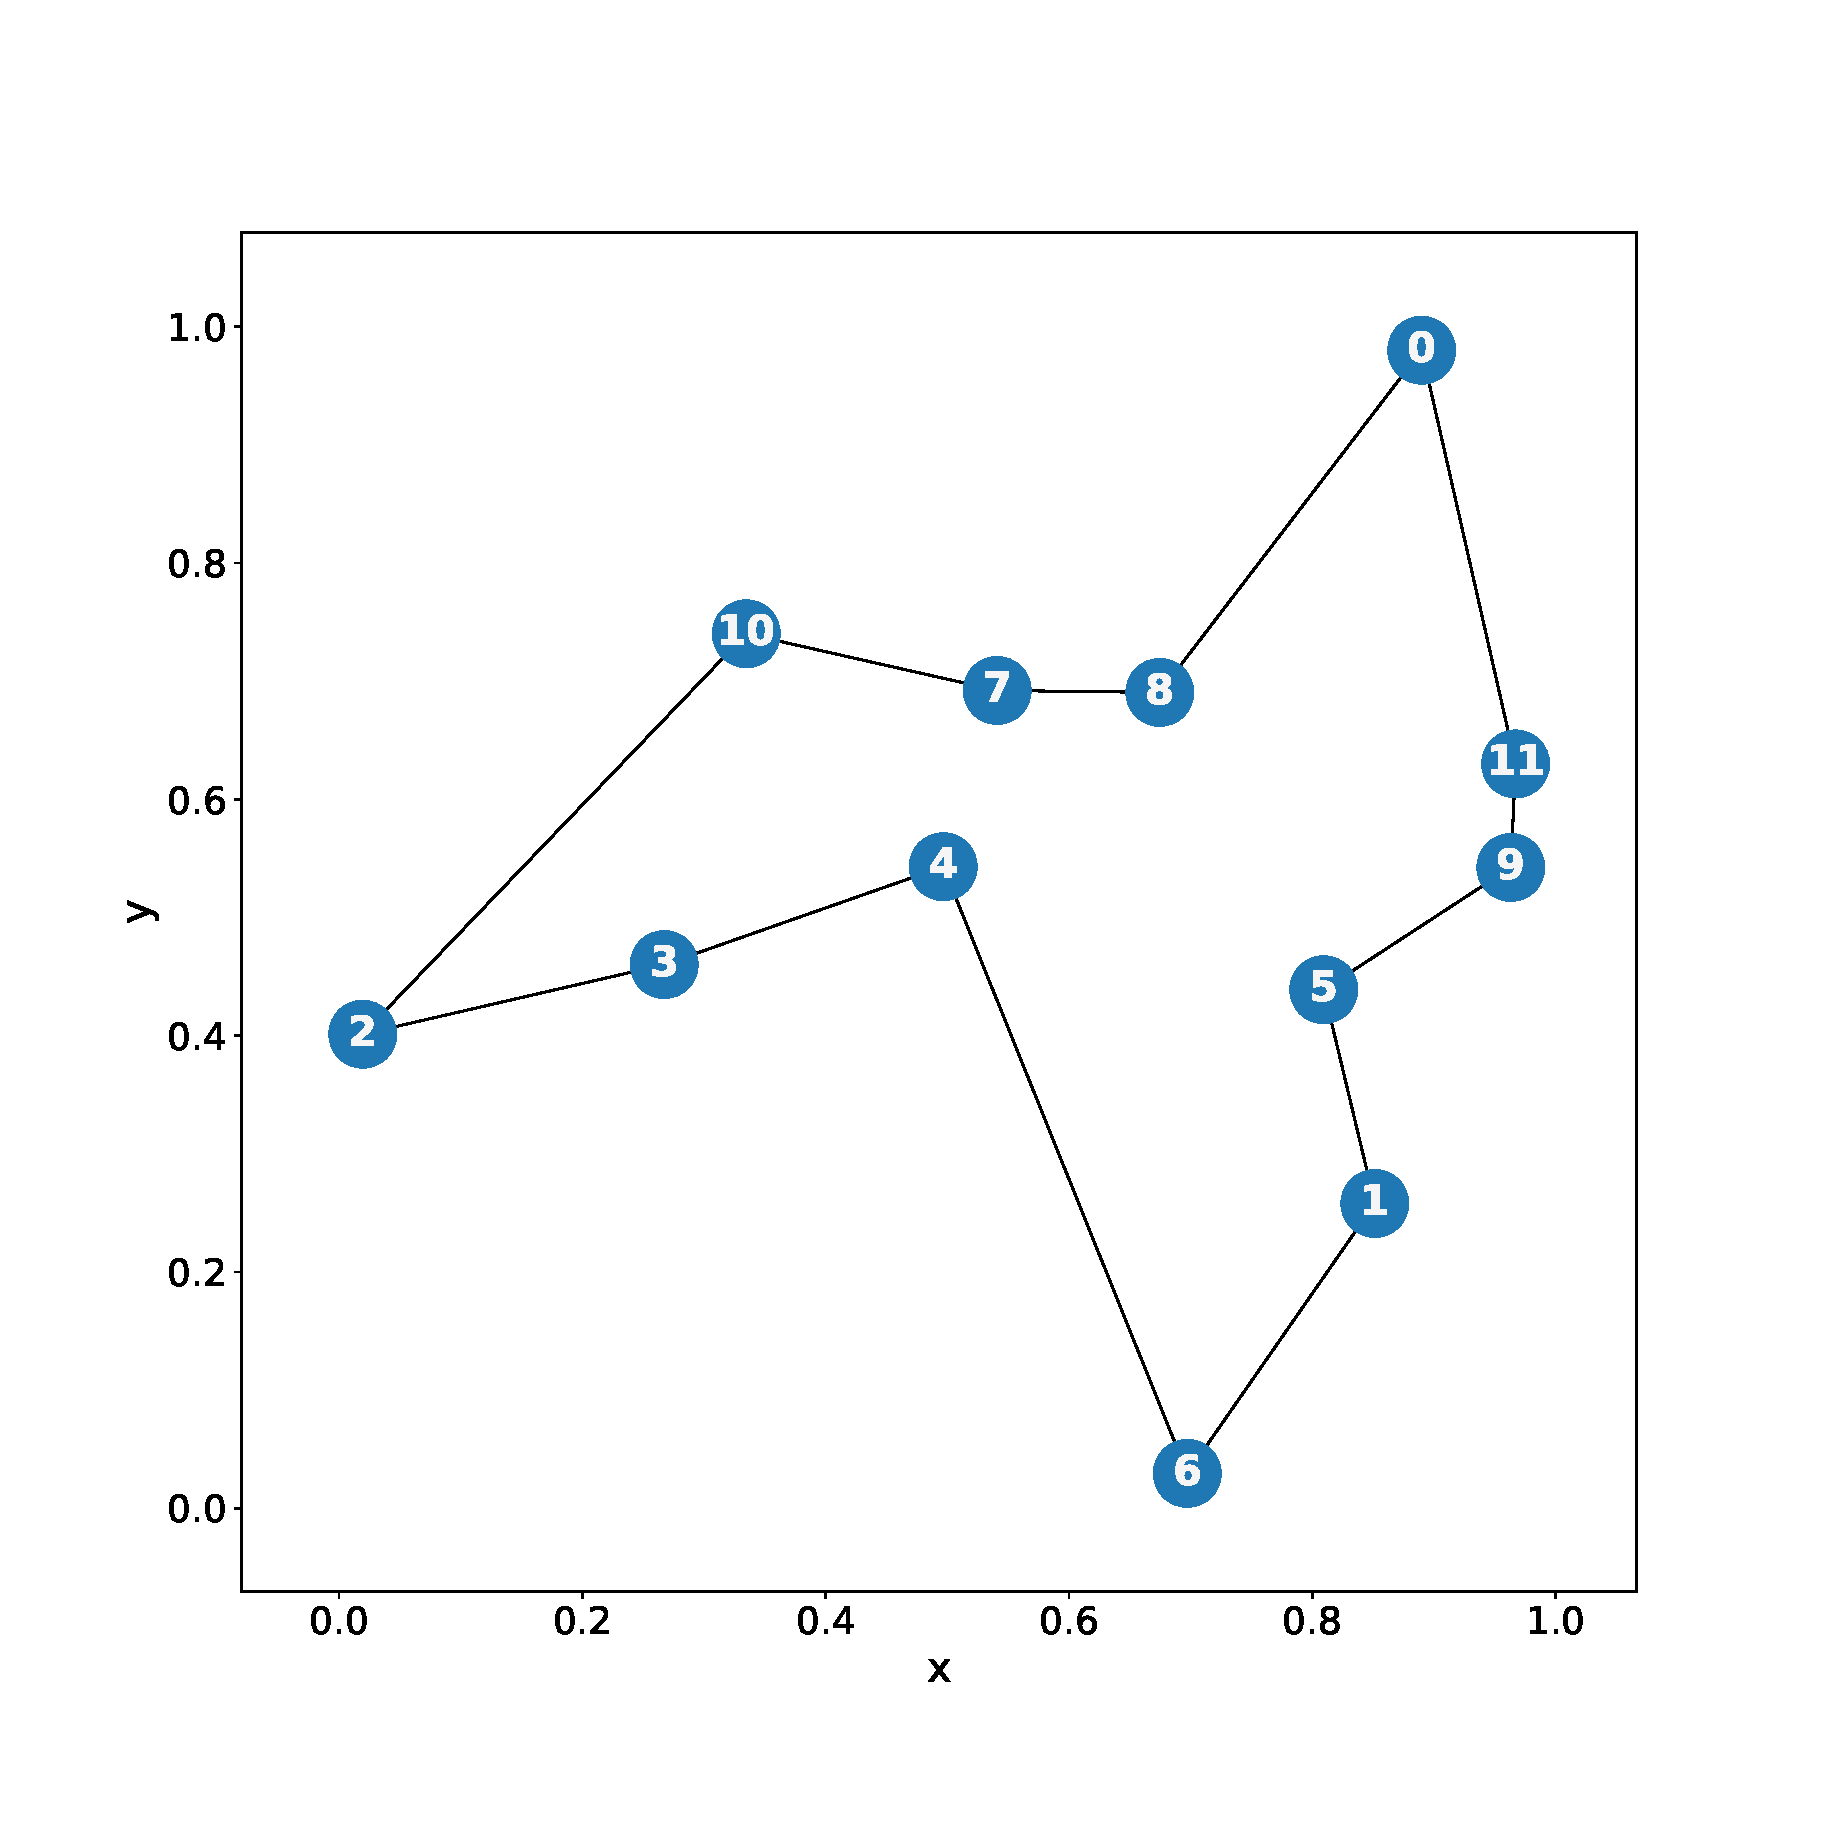
\includegraphics[width=0.7\linewidth]{f1.eps} 
  \caption{Tour associated with the best upper bound.}
  \label{f3}
\end{figure}

The complete list of successive tours with its associated cost is given in the Appendix. The python code used to implement the heuristic is shown below, Listing (\ref{ll2}).

\begin{code}
\captionof{listing}{Code section 2}
\label{ll2}
\pythoncode{2.py}
\end{code}

\section{Obtaining lower bounds}
Our goal is to solve the Symmetric Travelling Salesman Problem (P) over the complete graph built in the previous section
\begin{equation}
    \begin{aligned}
        \min \quad & \sum_{(i,j)\in E}c_{i,j}x_{i,j}\\
        \textrm{s.t.} \quad & \sum_{i<j}x_{i,j} + \sum_{j<i}x_{j,i} = 2 \quad \forall i \in V\\
        & \sum_{(i,j)\in S}x_{ij} \leq |S|-1 \quad \forall S \subset V\\
        & x_{i,j} \in \{0,1\} \quad \forall (i,j) \in E  \\
    \end{aligned}
    \tag{P}\label{opt-P}
\end{equation}
In previous section, we obtained several upper bounds for the problem by applying an heuristic procedure. In this section, we will solve some relaxations of problem (P) in order to obtain lower bounds.\\

In order to find lower bounds we will first solve the following linear relaxation (RP1) of the problem in which Subtour Elimination Constraints (SECs) are not taken into account.

\begin{equation}
    \begin{aligned}
        \min \quad & \sum_{(i,j)\in E}c_{i,j}x_{i,j}\\
        \textrm{s.t.} \quad & \sum_{i<j}x_{i,j} + \sum_{j<i}x_{j,i} = 2 \quad \forall i \in V\\
        & 0 \leq x_{i,j}\leq 1    \\
    \end{aligned}
    \tag{RP1}\label{opt-P}
\end{equation}

Afterwards, we will firstly add to problem (RP1) a violated SEC and solve the new relaxed problem (RP2). Secondly, we will add to problem (RP2) a violated valid inequality (different from SECs) and solve the new relaxed problem (RP3). Thirdly, we will add to problem (RP3) a gomory cut and solve the new relaxed problem (RP4). Finally, we will add to problem (RP4) a new violated SEC and solve the new relaxed problem (RP5).\\

We notice that the problem could be solved by only adding SECs to the initial problem formulation (RP1). However, we have decided to apply three different procedures (SEC, valid inequality and gomory cut) to improve the lower bound so as to have a better understanding of those procedures.\\

In order to solve the different relaxed problems we have used AMPL-CPLEX. However, in order to compute the gomory cut for problem (RP4) we have used the Python API for CPLEX.\\  

The following solution has been obtained for (RP1),

\begin{equation}
    x^{1*} = 
\resizebox{0.5\linewidth}{!}{$
        \left[ \begin {array}{cccccccccccc} 
        
         0& 0& 0& 0& 0& 0& 0&  0& 1& 0& 0& 1\\
         0&0&0&0&0&1/2&1&0&0&1/2&0&0\\
         0&0&0&1&0&0&0&0&0&0&1&0\\
         0&0&0&0&1/2&0&0&0&0&0&1/2&0\\
         0&0&0&0&0&0&0&1&0&0&1/2&0\\
         0&0&0&0&0&0&1&0&0&1/2&0&0\\
         0&0&0&0&0&0&0&0&0&0&0&0\\
         0&0&0&0&0&0&0&0&1&0&0&0\\
         0&0&0&0&0&0&0&0&0&0&0&0\\
         0&0&0&0&0&0&0&0&0&0&0&1\\
         0&0&0&0&0&0&0&0&0&0&0&0\\
         0&0&0&0&0&0&0&0&0&0&0&0\\
        \end {array}
        \right]     
$}
\text{, } \quad z^{1*} = 3.249
\end{equation}

Figure (\ref{f4}) shows the graphical solution of (RP1). As it can be seen, the solution of problem (RP1) is not a solution for the original TSP problem.

\begin{figure}[H]
\centering
    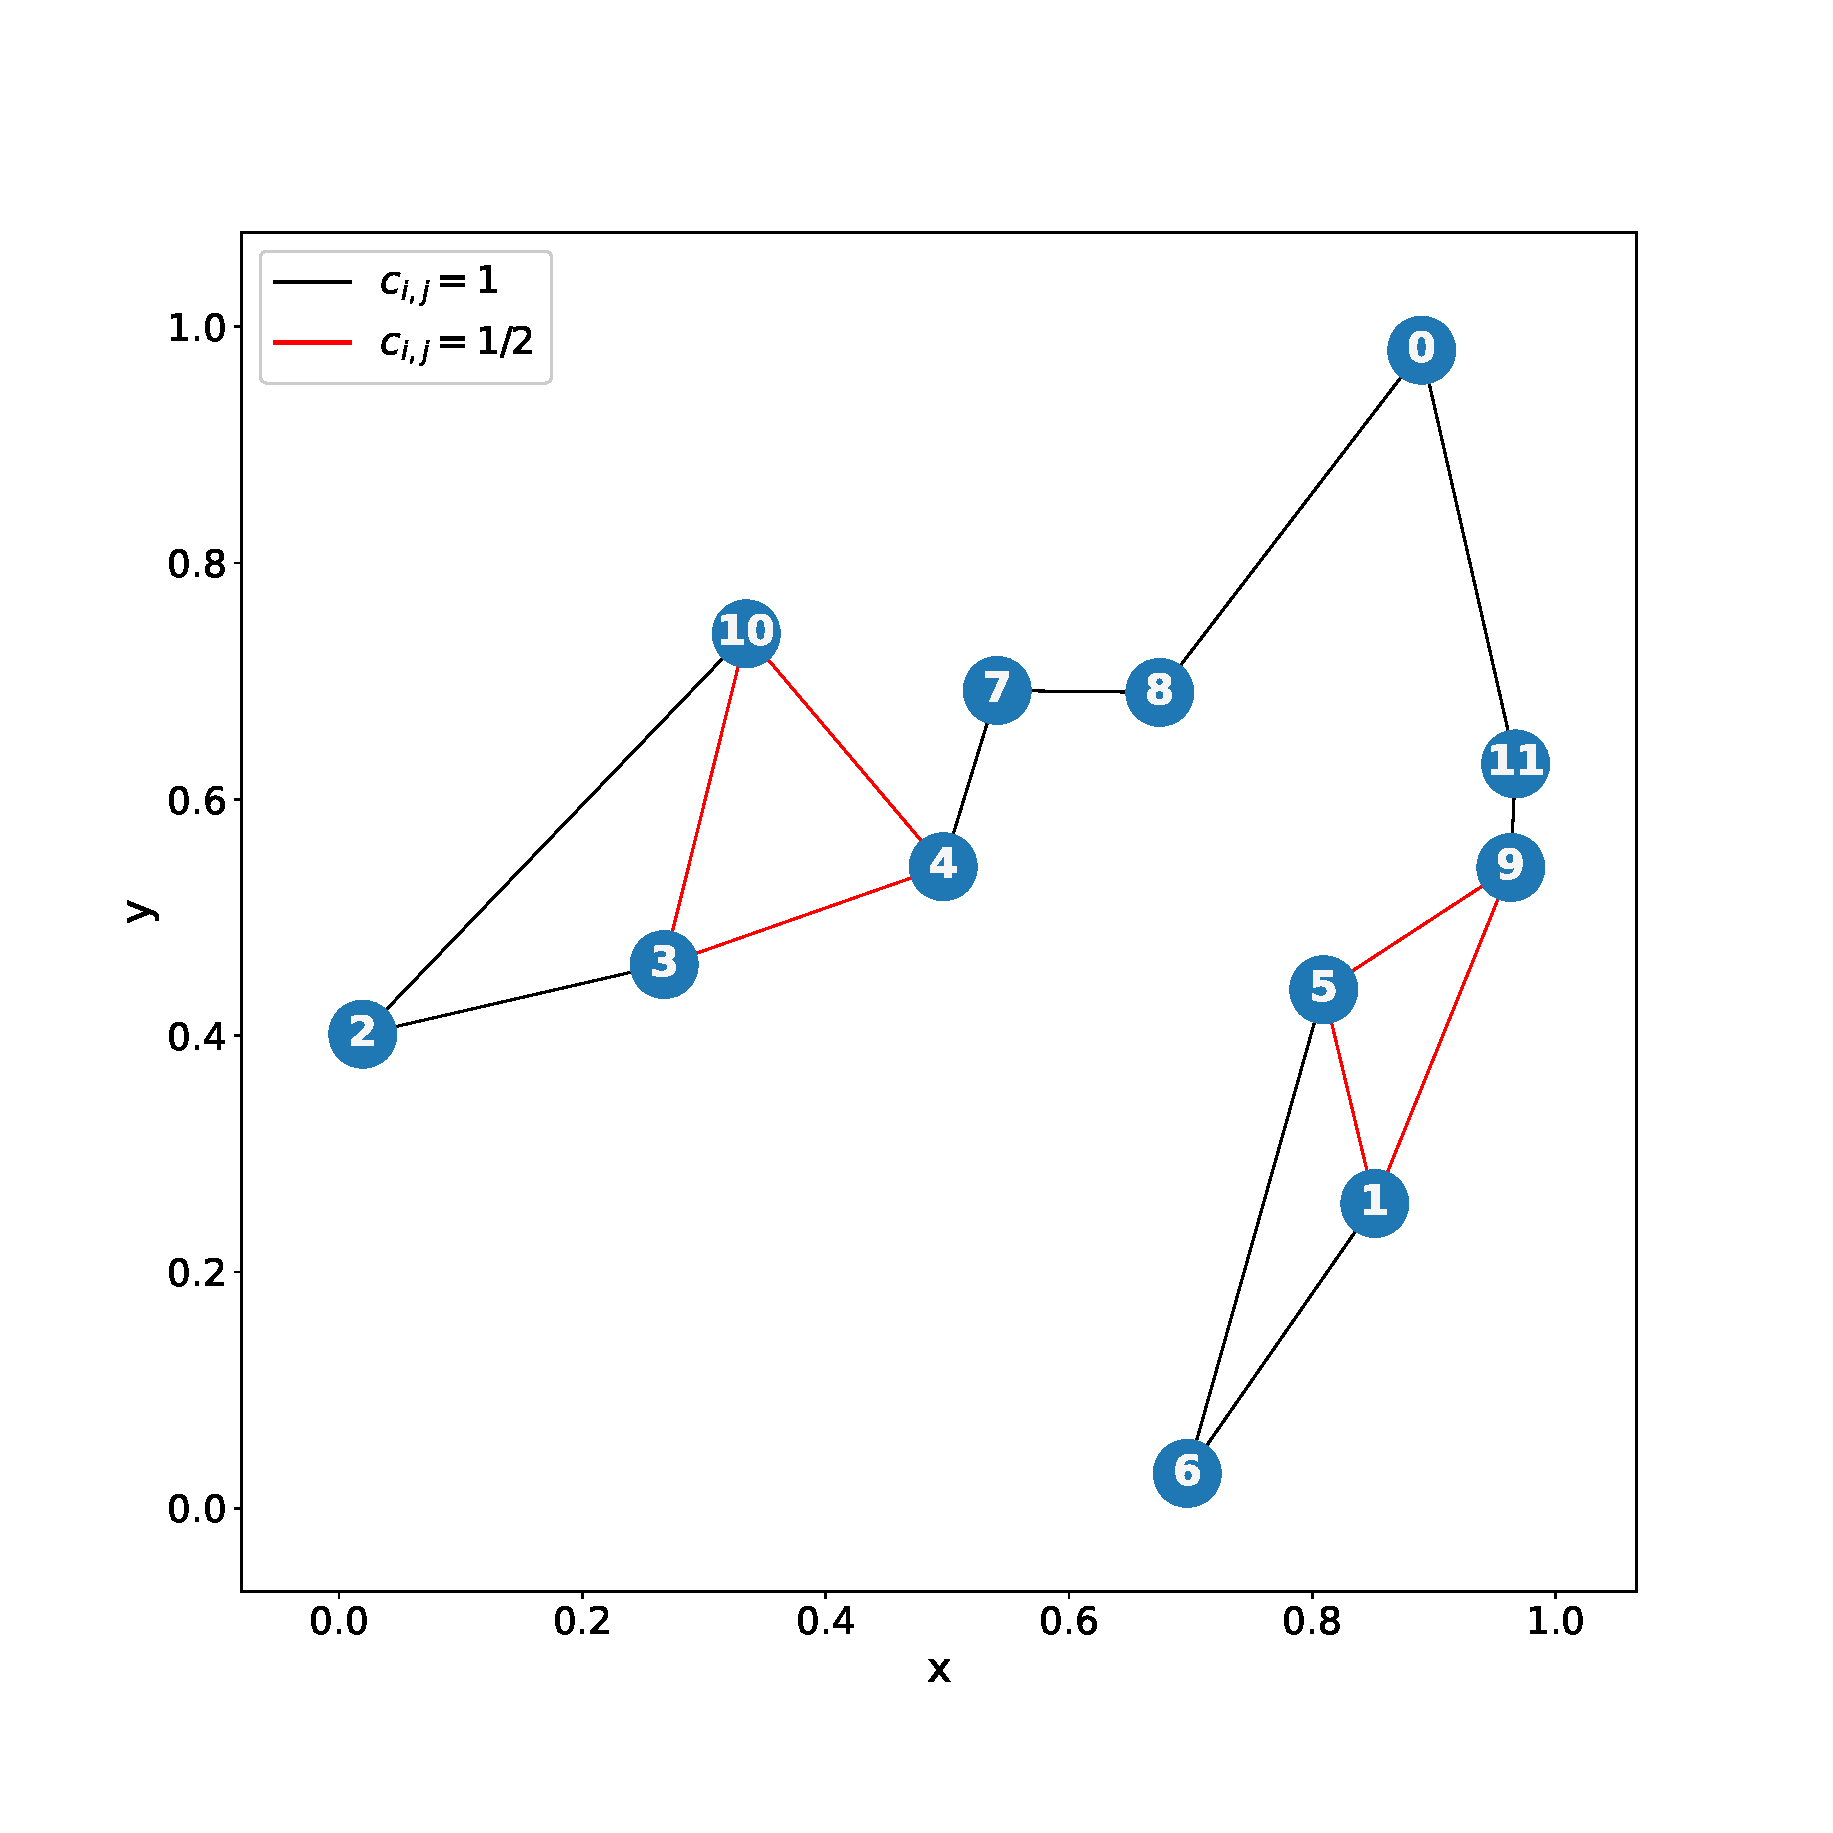
\includegraphics[width=0.7\linewidth]{f2.eps} 
  \caption{(RP1) solution}
  \label{f4}
\end{figure}

\subsection{First Subtour Elimination Constraint (SEC-1)}
We look for a Subtour Elimination Constraint (SEC) violated by $x^{1*}$ and add it to the formulation of (RP1). In order to find it we will use the SEC identification heuristic method.\\

\textbf{SEC identification heuristic method:} Let $x^{*}$ be the current solution and $G(x^{*})$ the graph induced by $x^{*}$.
\begin{enumerate}
    \item If there exist $(i,j)$ such that $x_{i,j}^{*}>1$, then the nodes involved in $(i,j)$ define the SEC violated by $x^{*}$.
    \item Else if $x_{i,j}^{*} < 1,  \forall (i,j) \in G(x^{*})$, then there are not violated SEC in the graph detected by the heuristic method.
    \item Else if there exists $(i,j)$ such that $x_{i,j}^{*} = 1$ then we generate a pseudo-node $\hat{i}_{i,j}$ that results from aggregating i and j and
    \begin{itemize}
        \item If for some node k, $x_{i,k}^{*}>0$ and $x_{j,k}^{*}>0$ then we create an edge $(\hat{i}_{i,j},k)$ with value $x_{\hat{i}_{i,j},k}^{*} = x_{i,k}^{*}+x_{j,k}^{*}$.
        \item If for some node k, $x_{i,k}^{*}>0$ or $x_{j,k}^{*}>0$ then we create an edge $(\hat{i}_{i,j},k)$ with value $x_{\hat{i}_{i,j},k}^{*} = x_{i,k}^{*}$ or $ x_{\hat{i},k}^{*} = x_{j,k}^{*}$.
    \end{itemize}
\end{enumerate}

Applying the SEC identification heuristic method to $G(x^{1*})$ we observe that the subset $S_{1} = \{2,3,10\} \subset V$ define a SEC violated by $x^{1*}$: if we consider the pseudo-node resulting from aggregating nodes 2 and 3, $\hat{i}_{2,3}$, we observe that the edge $(\hat{i}_{2,3},10)$ has $x_{\hat{i}_{2,3},10}^{*} = 1.5 > 1$. \\

Therefore, the SEC violated by $x^{1*}$ and given by $S_{1}$ (SEC-1) is

\begin{equation}
    \sum_{\substack{(i,j) \in S_{1}\\i<j}}x_{i,j} \leq |S_{1}|-1  \tag{SEC-1}
\end{equation}

We add (SEC-1) to the formulation of (RP1) obtaining (RP2)

\begin{equation}
    \begin{aligned}
        \min \quad & \sum_{(i,j)\in E}c_{i,j}x_{i,j}\\
        \textrm{s.t.} \quad & \sum_{i<j}x_{i,j} + \sum_{j<i}x_{j,i} = 2 \quad \forall i \in V\\
        & (\text{SEC-1})   \\
        & 0 \leq x_{i,j}\leq 1    \\
    \end{aligned}
    \tag{RP2}\label{opt-P2}
\end{equation}

The following solution has been obtained for (RP2),

\begin{equation}
    x^{2*} = 
\resizebox{0.5\linewidth}{!}{$
        \left[ \begin {array}{cccccccccccc} 
        
         0& 0& 0& 0& 0& 0& 0&  0& 1& 0& 0& 1\\
         0&0&0&0&0&1/2&1&0&0&1/2&0&0\\
         0&0&0&1&0&0&0&0&0&0&1&0\\
         0&0&0&0&1&0&0&0&0&0&0&0\\
         0&0&0&0&0&0&0&1/2&0&0&1/2&0\\
         0&0&0&0&0&0&1&0&0&1/2&0&0\\
         0&0&0&0&0&0&0&0&0&0&0&0\\
         0&0&0&0&0&0&0&0&1&0&1/2&0\\
         0&0&0&0&0&0&0&0&0&0&0&0\\
         0&0&0&0&0&0&0&0&0&0&0&1\\
         0&0&0&0&0&0&0&0&0&0&0&0\\
         0&0&0&0&0&0&0&0&0&0&0&0\\
        \end {array}
        \right]     
$}
\text{, } \quad z^{2*} = 3.255
\end{equation}

Figure (\ref{f5}) shows the graphical solution of (RP2).
\begin{figure}[H]
\centering
    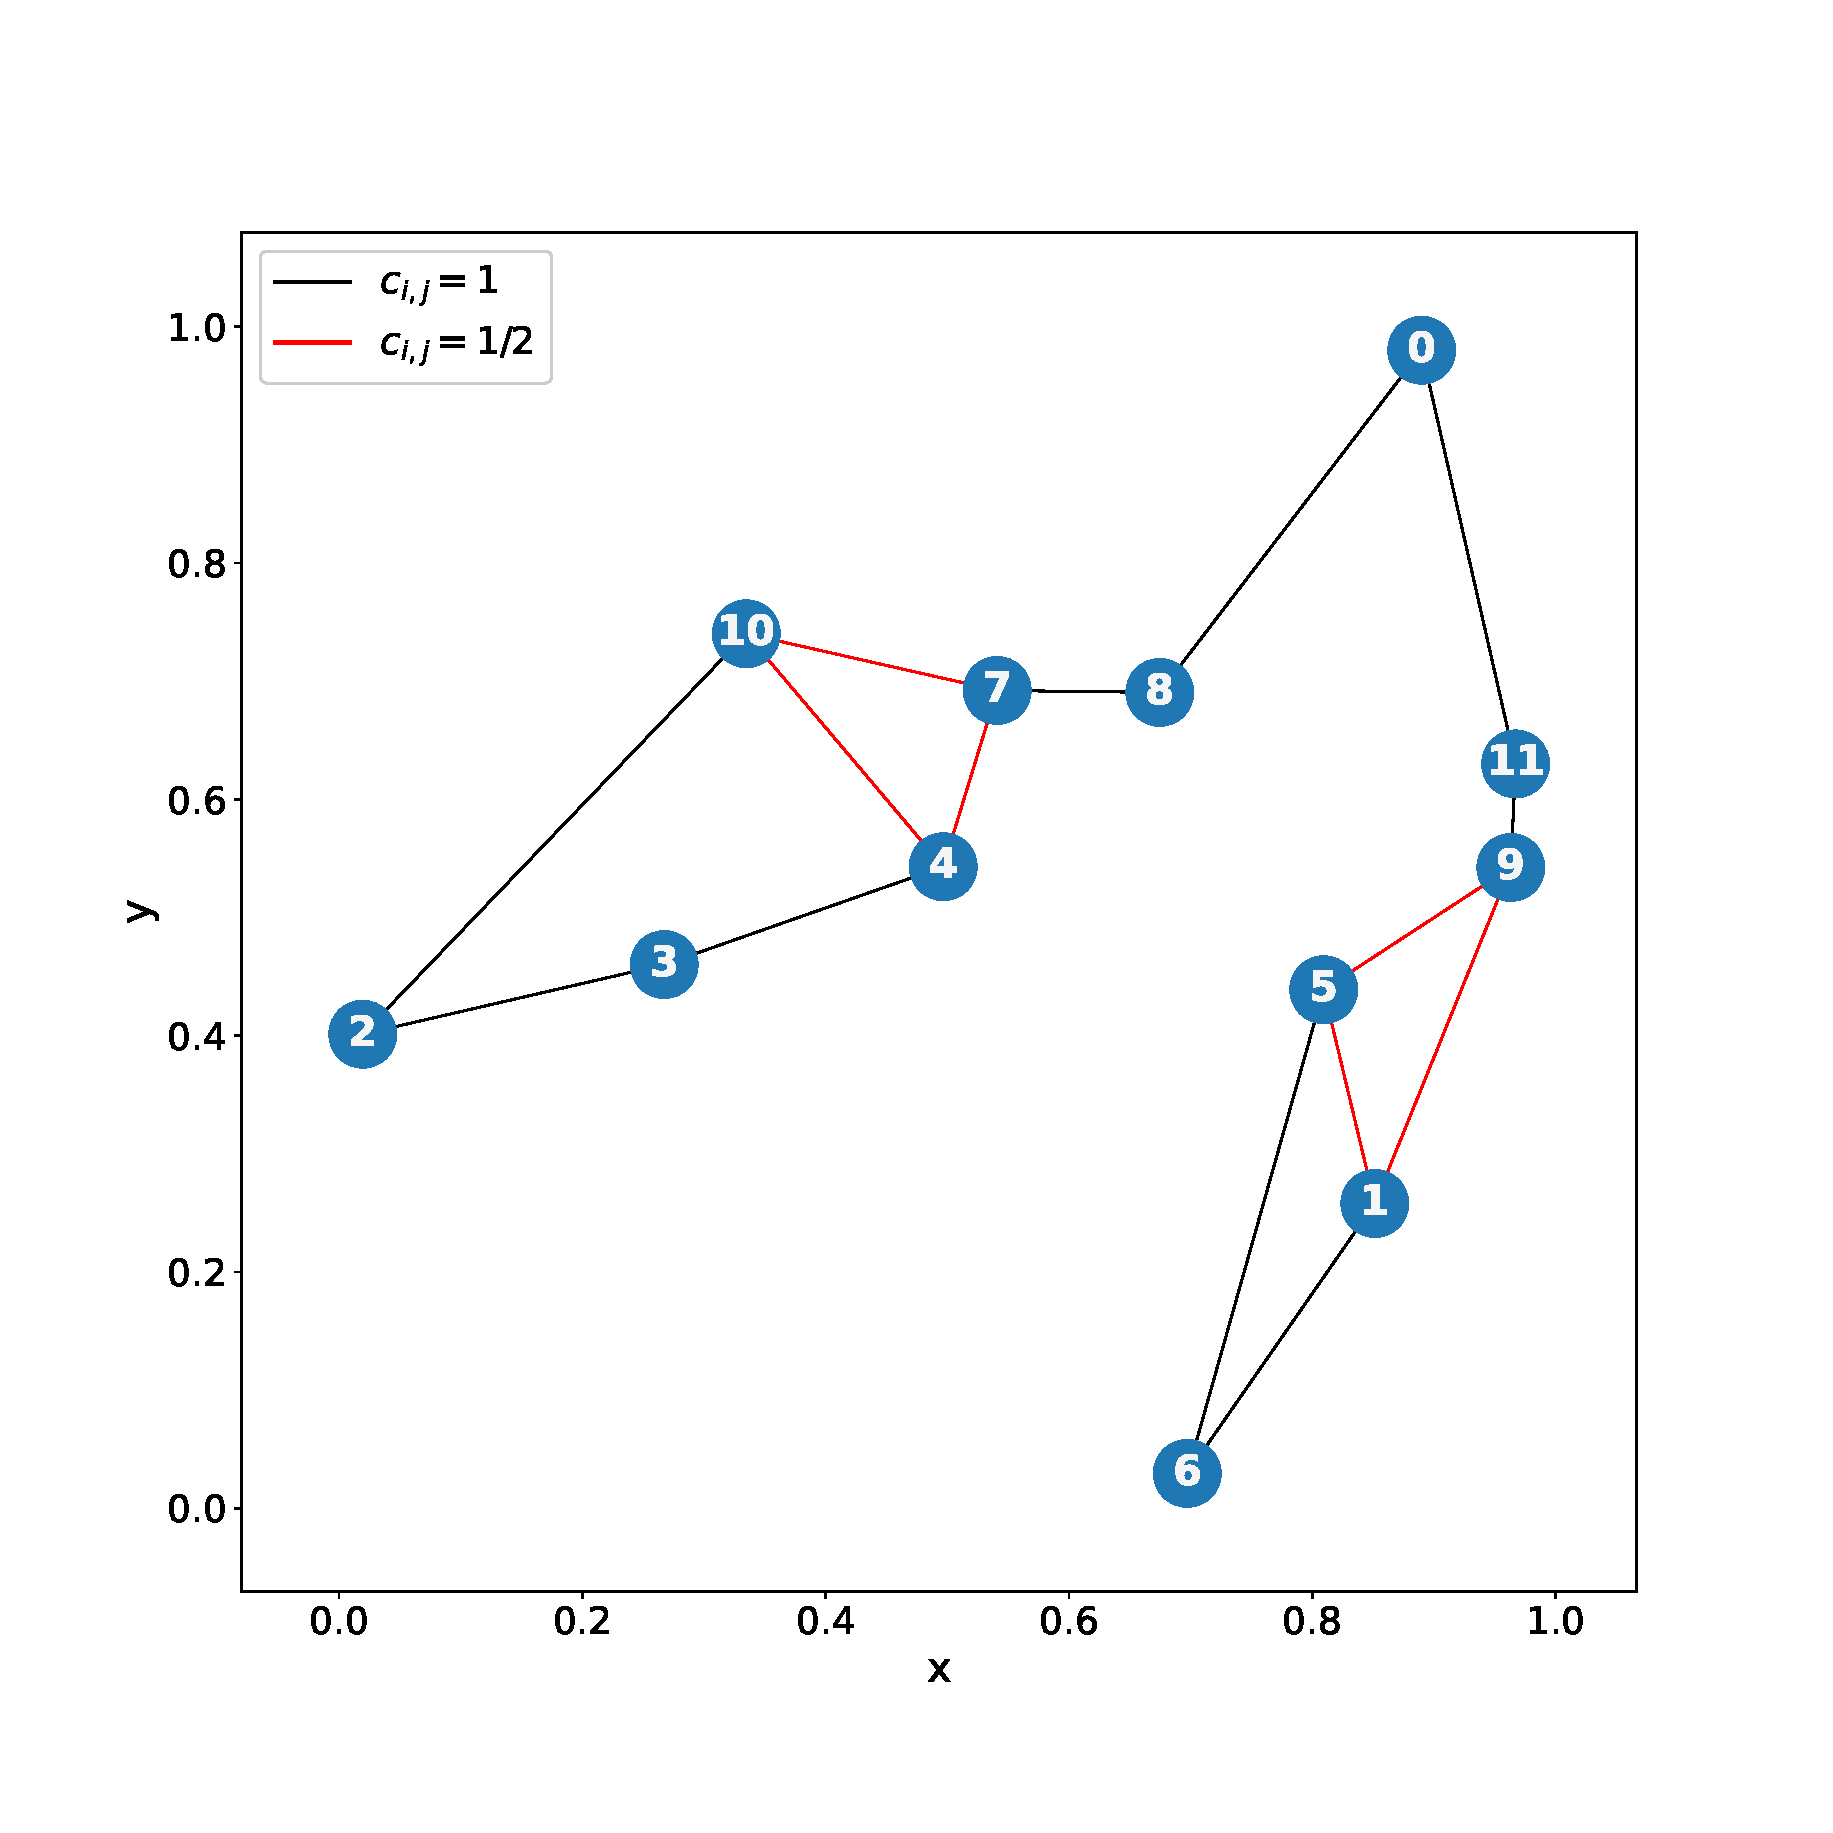
\includegraphics[width=0.7\linewidth]{f6.eps} 
  \caption{(RP2) solution}
  \label{f5}
\end{figure}
Again, solution to (RP2) is still not being a solution to the original TSP problem.

\subsection{Valid Inequality (different from SECs)}
Now we look for some valid inequality for the TSP (different from the SEC's) which be violated by $x^{2*}$. In order to find it, we will compute a Chvátal-Gomory inequality violated by $x^{2*}$. \\

\textbf{Step 1:}
We sum up the degree equations for the set of nodes in $H = \{1,5,9\}$.
Let $c(i)$ be the degree equation associated with node $i$, that is
\begin{equation}
    c(i): \sum_{i<j}x_{ij} + \sum_{j<i}x_{ji} = 2 
\end{equation}

Then, we have

\begin{equation}
   c(1)+c(5)+c(9) = 2\times3
   \label{eq8}
\end{equation}

\textbf{Step 2:}
Since, all variables $x_{ij}$ satisfy $0 \leq x_{ij}\leq 1$, then from Eq. (\ref{eq8}) we have the inequality

\begin{equation}
   2\sum_{\substack{(i,j) \in H\\i<j}}x_{i,j} + x_{1,6}+x_{5,6}+x_{9,11} \leq 2\times3
   \label{eq9}
\end{equation}

\textbf{Step 3:}
We sum to Eq. (\ref{eq9}) the inequalities (upper bounds)
\begin{equation}
    x_{1,6} \leq 1, \quad x_{5,6} \leq 1, \quad x_{9,11} \leq 1
\end{equation}
and we obtain the following inequality
\begin{equation}
   2\sum_{\substack{(i,j) \in H\\i<j}}x_{i,j} + 2(x_{1,6}+x_{5,6}+x_{9,11}) \leq 2\times3 + 3
   \label{eq100}
\end{equation}
Multiplying Eq. (\ref{eq100}) by 1/2 and since

\begin{equation}
    \sum_{\substack{(i,j) \in H\\i<j}}x_{i,j} = x_{1,5} + x_{1,9} + x_{5,9}
\end{equation}
we obtain
\begin{equation}
   x_{1,5} + x_{1,9} + x_{5,9} + x_{1,6}+x_{5,6}+x_{9,11} \leq 3 + 3/2
   \label{eq10}
\end{equation}
Now, since the the left hand side for the TSP should be integer-valued we can round down the right hand side to obtain a valid inequality for the STP, which in fact is violated by $x^{2*}$ ($4.5 > 4$)
\begin{equation}
   x_{1,5} + x_{1,9} + x_{5,9} + x_{1,6}+x_{5,6}+x_{9,11} \leq 4 \tag{INEQ-1}
   \label{eq10}
\end{equation}
Therefore, we add (INEQ-1) to the formulation of (RP2) in order to obtain (RP3).\\

\begin{equation}
    \begin{aligned}
        \min \quad & \sum_{(i,j)\in E}c_{i,j}x_{i,j}\\
        \textrm{s.t.} \quad & \sum_{i<j}x_{i,j} + \sum_{j<i}x_{j,i} = 2 \quad \forall i \in V\\
        & (\text{SEC-1})    \\
        & (\text{INEQ-1}) \\
        & 0 \leq x_{i,j}\leq 1   \\
    \end{aligned}
    \tag{RP3}\label{opt-P2}
\end{equation}

The following solution has been obtained for (RP3),

\begin{equation}
    x^{3*} = 
\resizebox{0.5\linewidth}{!}{$
        \left[ \begin {array}{cccccccccccc} 
        
         0&0&0&0&0&0&0&0&1&0&0&1\\
         0&0&0&0&0&1&1&0&0&0&0&0\\
         0&0&0&1&0&0&0&0&0&0&1&0\\
         0&0&0&0&1&0&0&0&0&0&0&0\\
         0&0&0&0&0&0&0&1/2&0&0&1/2&0\\
         0&0&0&0&0&0&1/2&0&0&1/2&0&0\\
         0&0&0&0&0&0&0&0&0&1/2&0&0\\
         0&0&0&0&0&0&0&0&1&0&1/2&0\\
         0&0&0&0&0&0&0&0&0&0&0&0\\
         0&0&0&0&0&0&0&0&0&0&0&1\\
         0&0&0&0&0&0&0&0&0&0&0&0\\
         0&0&0&0&0&0&0&0&0&0&0&0\\
        \end {array}
        \right]     
$}
\text{, } \quad z^{3*} = 3.2715
\end{equation}

Figure (\ref{ff7}) shows the graphical solution of (RP3).
\begin{figure}[H]
\centering
    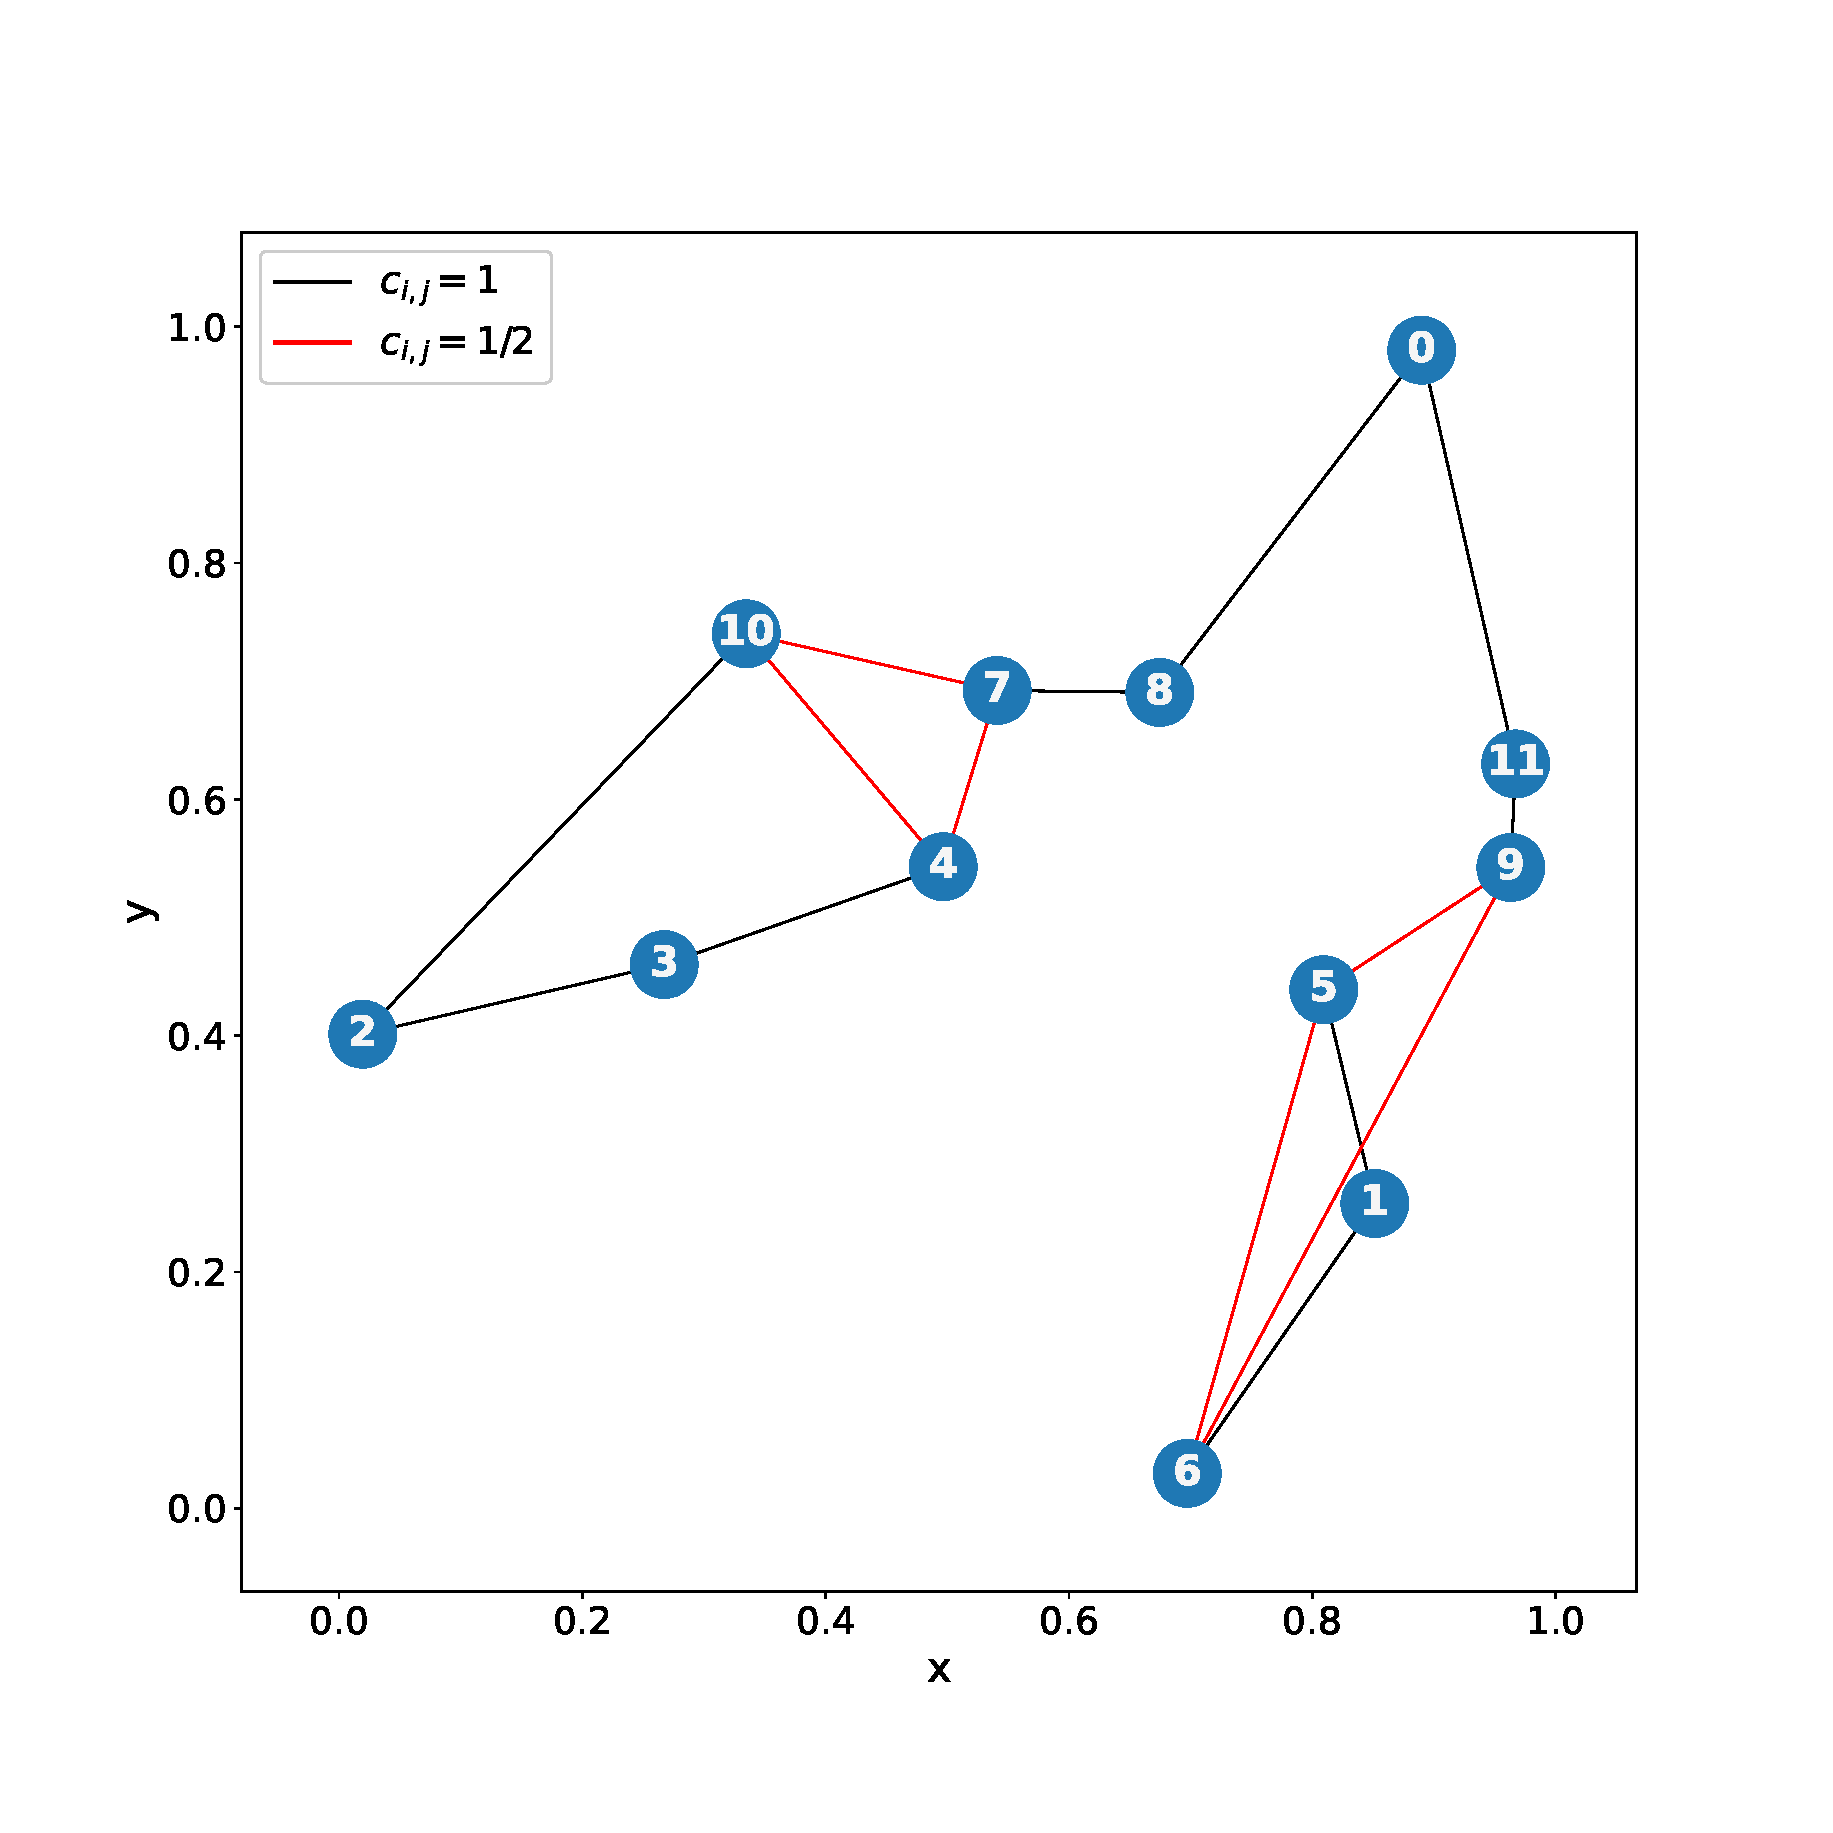
\includegraphics[width=0.7\linewidth]{f8.eps} 
  \caption{(RP3) solution}
  \label{ff7}
\end{figure}
Again, solution to (RP3) is still not being a solution to the original TSP problem.

\subsection{Gomory Cut}
Now, we try to identify some Gomory cut violated by $x^{3*}$. In order to compute it, we have used the Python API for CPLEX and intance methods \textit{binvarow()} and \textit{basis.write()} which provide the $i-th$ row of the optimal LP tableau and basic variables information, respectively.\\

In order to use the Python API for CPLEX we have firstly export the AMPL model into a \textit{.mps} format file (Appendix: tsp.mps). The code below, Listing (\ref{ll3}) shows the python code used.

\begin{code}
\captionof{listing}{Code section 3 (Gomory cut)}
\label{ll3}
\pythoncode{p11.py}
\end{code}

We will compute the gomory cut associated with the basic variable $x_{5,8}$ which has a non-integer value ($x_{5,8}^{3*} = 1/2$). The $8$-row is the one associated with basic variable $x_{5,8}$ (Appendix: .col + basis.mps). Then, according to the Tableau, the following equality must be satisfied by any feasible solution (in particular by $x^{3*}$)

\begin{equation}
\begin{split}
    x_{5,8} -\frac{1}{2}(x_{1,3}+x_{1,4}+x_{1,11}+x_{2,3}+x_{2,4}+x_{2,11}+ x_{3,6}+x_{3,7}+x_{3,9}+x_{3,10}+x_{3,12}+x_{4,6}+x_{4,7}+\\+x_{4,9}+x_{4,10}+x_{4,12}+ x_{6,11}+x_{7,11}+x_{9,11}+x_{10,11}+x_{11,12}) +\\ +\frac{1}{2}(x_{1,5}+x_{1,8}+x_{2,5}+x_{2,8}+x_{5,6}+x_{5,7}+x_{5,9}+x_{5,10}+x_{5,12}+x_{6,8}++x_{7,8}+x_{8,9}+x_{8,10}+x_{8,12}) \\ = 1/2
\end{split}
\label{eq19}
\end{equation}

In order to compute the Gomory cut (GC-1), we notice that variables $x_{i,j}$ are integer and non-negative and we round down the right hand side and coefficients on the left hand side and we obtain,

\begin{equation}
\begin{split}
    x_{5,8} -\frac{1}{2}(x_{1,3}+x_{1,4}+x_{1,11}+x_{2,3}+x_{2,4}+x_{2,11}+ x_{3,6}+x_{3,7}+x_{3,9}+x_{3,10}+x_{3,12}+x_{4,6}+x_{4,7}+\\+x_{4,9}+x_{4,10}+x_{4,12}+
    x_{6,11}+x_{7,11}+x_{9,11}+x_{10,11}+x_{11,12}) \leq 0
\end{split}
\tag{GC-1}
\end{equation}

Therefore, we add (GC-1) to the formulation of (RP3) in order to obtain (RP4).

\begin{equation}
    \begin{aligned}
        \min \quad & \sum_{(i,j)\in E}c_{i,j}x_{i,j}\\
        \textrm{s.t.} \quad & \sum_{i<j}x_{i,j} + \sum_{j<i}x_{j,i} = 2 \quad \forall i \in V\\
        & (\text{SEC-1})    \\
        & \text{(INEQ-1)} \\
        & \text{(GC-1)} \\
        & 0 \leq x_{i,j}\leq 1   \\
    \end{aligned}
    \tag{P3}\label{opt-P2}
\end{equation}

The following solution has been obtained to (RP4), (Appendix: .sol)

\begin{equation}
    x^{4*} = 
\resizebox{0.5\linewidth}{!}{$
        \left[ \begin {array}{cccccccccccc} 
        
         0&0&0&0&0&0&0&0&1&0&0&1\\
         0&0&0&0&0&1&1&0&0&0&0&0\\
         0&0&0&1&0&0&1/3&0&0&0&2/3&0\\
         0&0&0&0&1&0&0&0&0&0&0&0\\
         0&0&0&0&0&0&&1/3&0&0&2/3&0\\
         0&0&0&0&0&0&1/3&0&0&2/3&0&0\\
         0&0&0&0&0&0&0&0&0&1/3&0&0\\
         0&0&0&0&0&0&0&0&1&0&2/3&0\\
         0&0&0&0&0&0&0&0&0&0&0&0\\
         0&0&0&0&0&0&0&0&0&0&0&1\\
         0&0&0&0&0&0&0&0&0&0&0&0\\
         0&0&0&0&0&0&0&0&0&0&0&0\\
        \end {array}
        \right]     
$}
\text{, } \quad z^{4*} = 3.29
\end{equation}

Figure (\ref{ff8}) shows the graphical solution of (RP4).
\begin{figure}[H]
\centering
    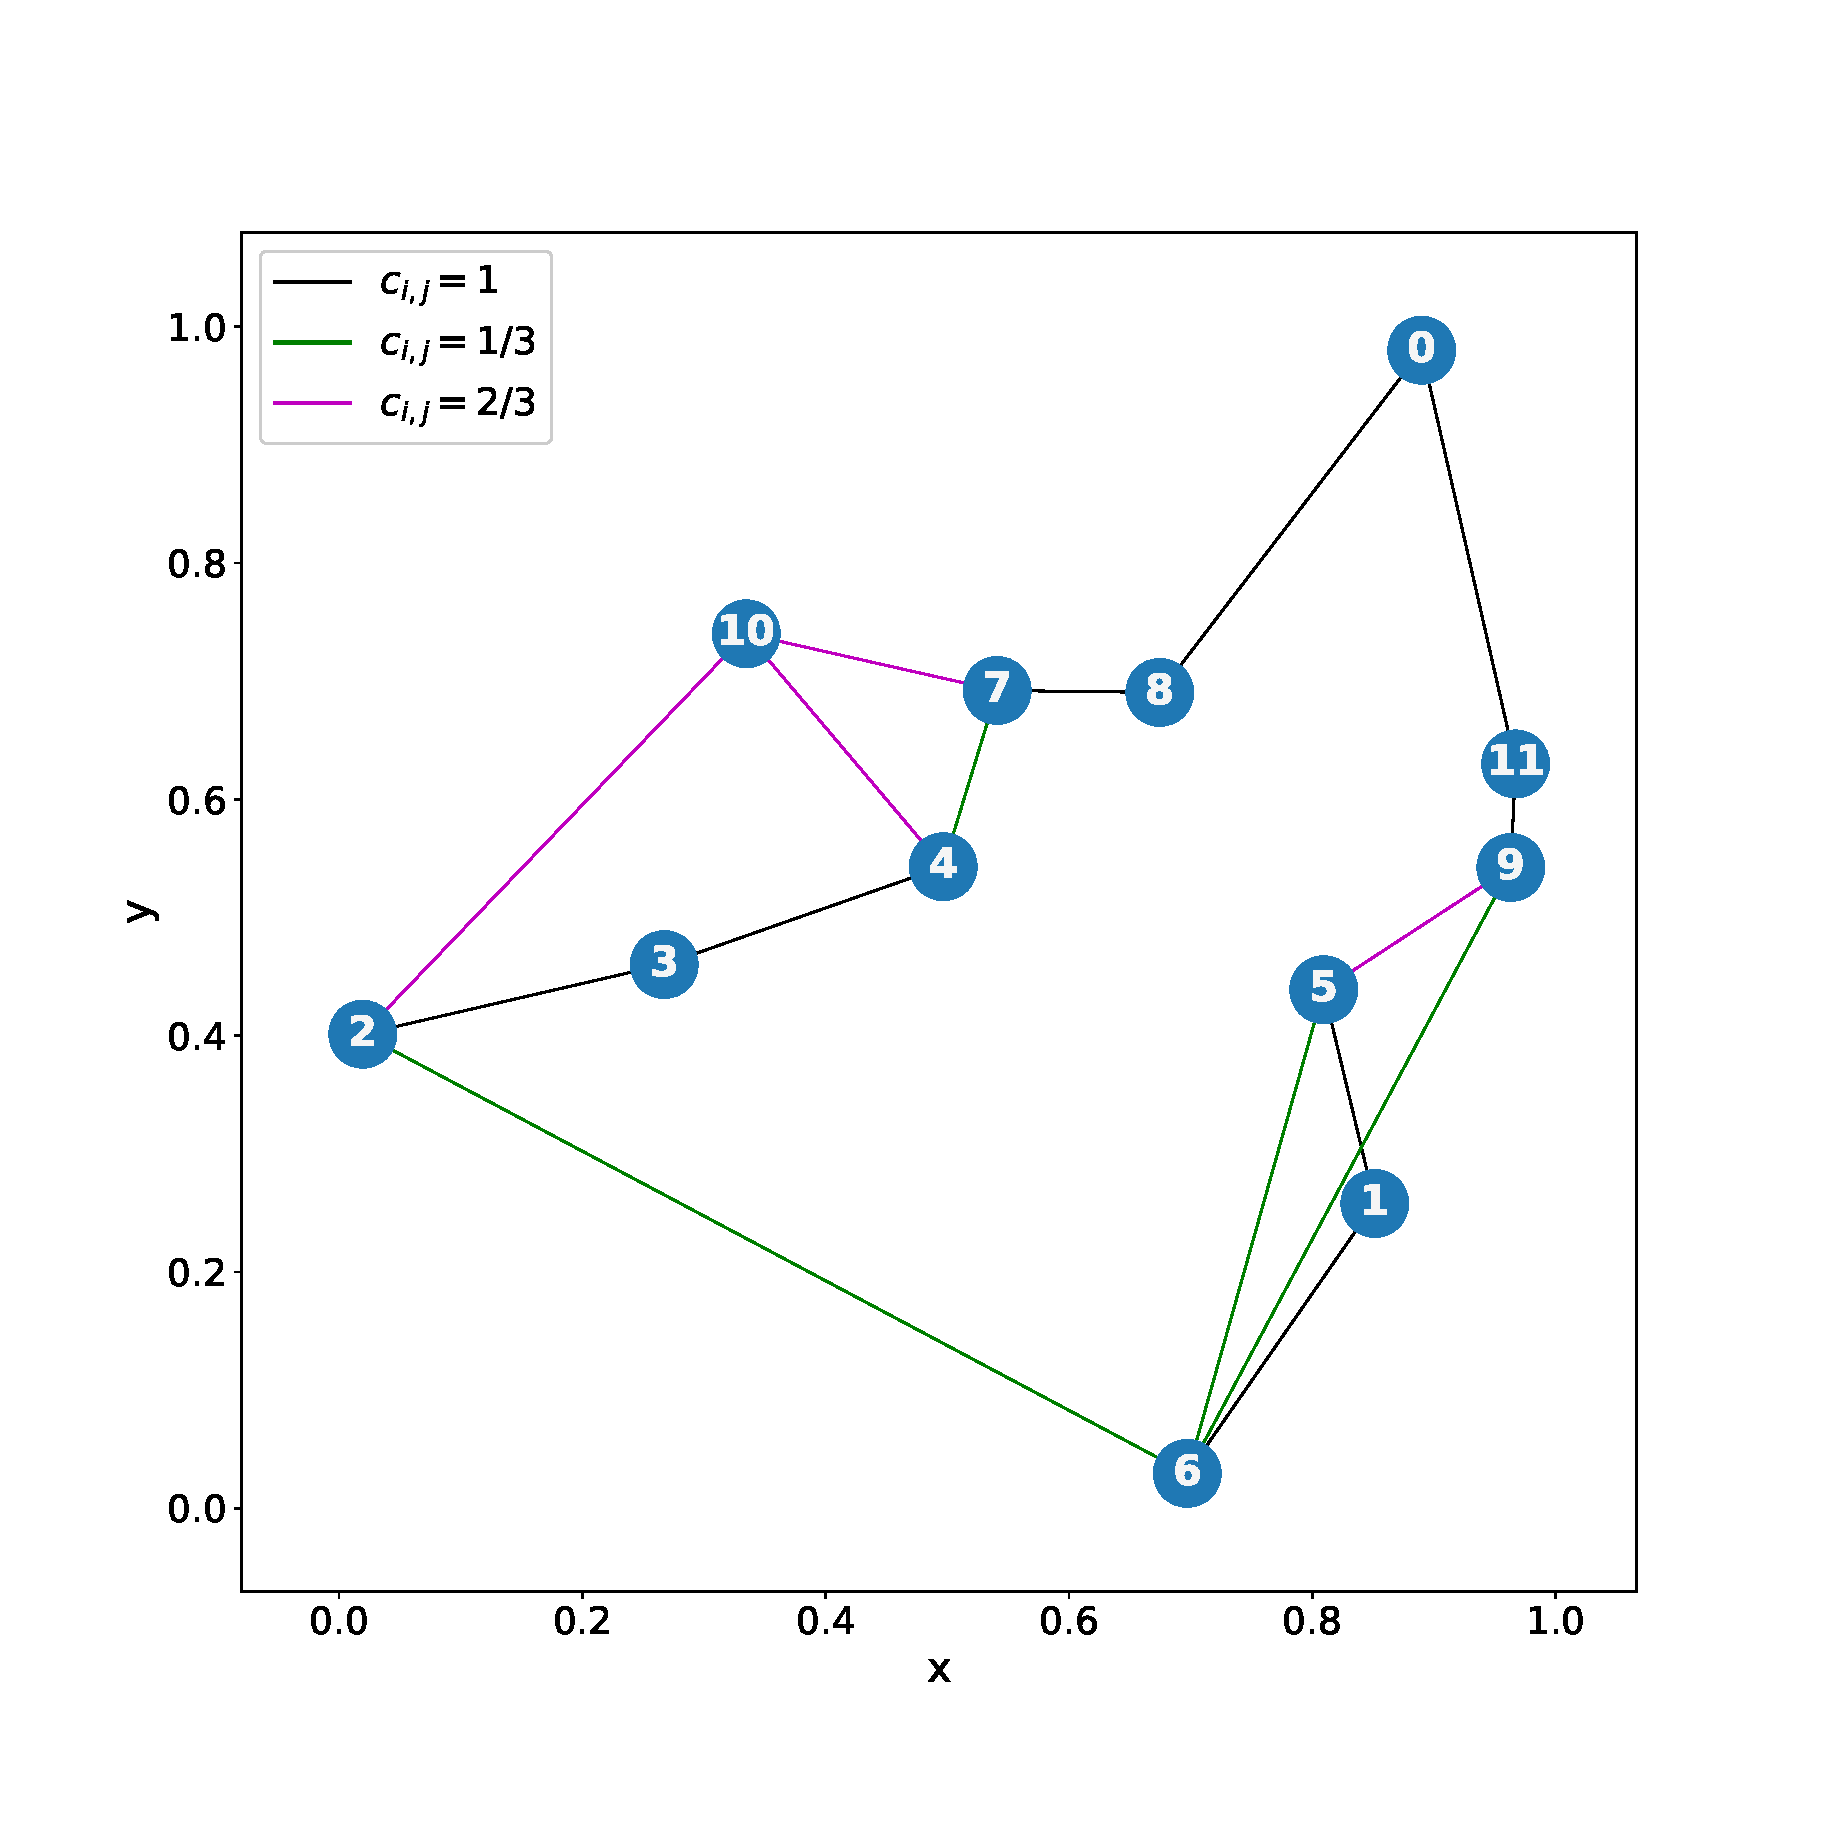
\includegraphics[width=0.7\linewidth]{ff1.eps} 
  \caption{(RP4) solution}
  \label{ff8}
\end{figure}
Again, solution to (RP4) is still not being a solution to the original TSP problem.

\subsection{Second Subtour Elimination constraint (SEC-2)}
We look for a Subtour Elimination Constraint (SEC) violated by $x^{4*}$ and add it to the formulation of (RP4).  In order to find it we will use the SEC identification heuristic method previously explained.\\

Applying the SEC identification heuristic method to $G(x^{4*})$ we observe that the subset $S_{2} = \{1,5,6\} \subset V$ defines a SEC violated by $x^{4*}$: if we consider the pseudo-node resulting from aggregating nodes 1 and 6, $\hat{i}_{1,6}$, we observe that the edge $(\hat{i}_{1,6},5)$ has $x_{\hat{i}_{1,6},5}^{*} = 1 + 1/3 > 1$. \\

Therefore, the SEC violated by $x^{4*}$ and given by $S_{2}$ (SEC-2) is

\begin{equation}
    \sum_{\substack{(i,j) \in S_{2}\\i<j}}x_{i,j} \leq |S_{2}|-1  \tag{SEC-2}
\end{equation}

We add (SEC-2) to the formulation of (RP4) obtaining (RP5)

\begin{equation}
    \begin{aligned}
        \min \quad & \sum_{(i,j)\in E}c_{i,j}x_{i,j}\\
        \textrm{s.t.} \quad & \sum_{i<j}x_{i,j} + \sum_{j<i}x_{j,i} = 2 \quad \forall i \in V\\
        & (\text{SEC-1})   \\
        & \text{(INEQ-1)} \\
        & \text{(GC-1)} \\
        & \text{(SEC-2)} \\
        & 0 \leq x_{i,j}\leq 1    \\
    \end{aligned}
    \tag{RP5}\label{opt-P2}
\end{equation}

The following solution has been obtained for (RP5),

\begin{equation}
    x^{5*} = 
\resizebox{0.4\linewidth}{!}{$
        \left[ \begin {array}{cccccccccccc} 
         0&0&0&0&0&0&0&0&1&0&0&1\\
         0&0&0&0&0&1&1&0&0&0&0&0\\
         0&0&0&1&0&0&0&0&0&0&1&0\\
         0&0&0&0&1&0&0&0&0&0&0&0\\
         0&0&0&0&0&0&1&0&0&0&0&0\\
         0&0&0&0&0&0&0&0&0&1&0&0\\
         0&0&0&0&0&0&0&0&0&0&0&0\\
         0&0&0&0&0&0&0&0&1&0&1&0\\
         0&0&0&0&0&0&0&0&0&0&0&0\\
         0&0&0&0&0&0&0&0&0&0&0&1\\
         0&0&0&0&0&0&0&0&0&0&0&0\\
         0&0&0&0&0&0&0&0&0&0&0&0\\
        \end {array}
        \right]     
$}
\text{, } \quad z^{5*} = 3.314
\end{equation}

Clearly, solution to (RP5) is the solution to the TSP as it is an integer solution and no SEC is violated. Moreover, for this solution the lower bound obtained equals the best upper bound obtained in the previous section

\begin{equation}
    z^{*} = \overline{z^{*}} = \underline{z^{*}}
\end{equation}
which shows optimality.\\

Figure (\ref{ff9}) shows the corresponding lower bounds for the TSP obtained in the relaxed problems (RP1), (RP2), (RP3), (RP4) and (RP5) just solved.

\begin{figure}[H]
\centering
    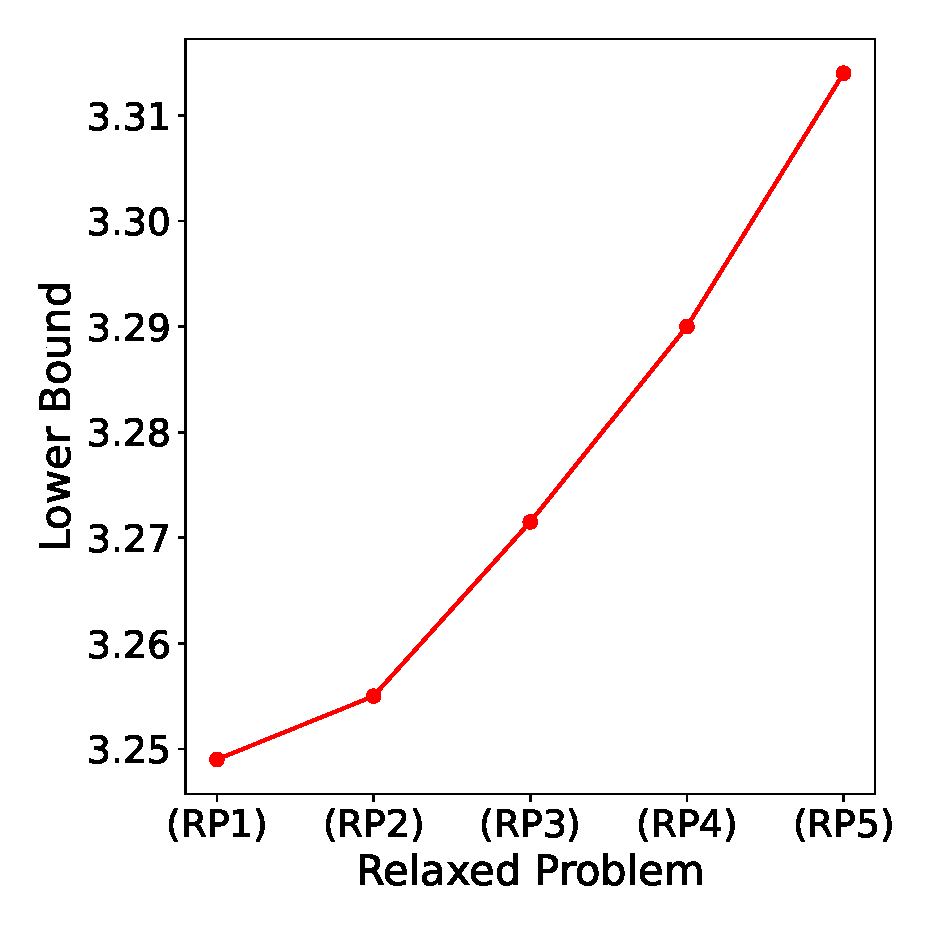
\includegraphics[width=0.45\linewidth]{ff2.eps} 
  \caption{TSP Lower bounds for the different relaxed problems solved.}
  \label{ff9}
\end{figure}

As expected, as the problem becomes more restrictive, lower bounds increase.\\

Below, we show the main AMPL-CPLEX files (.mod, .dat) used in this section.

\begin{code}
\captionof{listing}{Section 3 (.mod)}
\label{l1}
\begin{lstlisting}[basicstyle=\small]
# parameters
param n;
set nodes ordered := {1..n};
set edges := {i in nodes, j in nodes};

set nodes1 ordered := {3,4,11};
set edges1 := {i in nodes1, j in nodes1};

set nodes2 ordered := {2,6,7};
set edges2 := {i in nodes2, j in nodes2};

param c {(i,j) in edges};
var X {(i,j) in edges} >=0, <=1;

#Objective function
minimize fobj : sum {(i,j) in edges} (c[i,j]*X[i,j]);

#Constraints
subject to cc1 {i in nodes}: sum{(i,j) in edges: i < j} (X[i,j]) + sum{(i,j) in edges: j < i} (X[j,i])= 2; 
subject to cc2: sum{(i,j) in edges1:i < j} (X[i,j]) <= 2; 
subject to cc3: X[2,6]+X[2,10]+X[6,10]+X[2,7]+X[6,7]+X[10,12] <= 4; 
subject to cc4: X[5,8] - X[1,3]-X[1,4]-X[1,11]-X[2,3]-X[2,4]-X[2,11]-X[3,6]-X[3,7]-X[3,9]-X[3,10]-X[3,12]-X[4,6]-
-X[4,7]-X[4,9]-X[4,10]-X[4,12]-X[6,11]-X[7,11]-X[9,11]-X[10,11]-X[11,12] <= 0; 
subject to cc5: sum{(i,j) in edges2:i < j} (X[i,j]) <= 2; 

\end{lstlisting}
\end{code}

\begin{code}
\captionof{listing}{Section 3 (.dat)}
\label{l1}
\begin{lstlisting}[basicstyle=\small]
param n := 12;

param c: 1 2 3 4 5 6 7 8 9 10 11 12 :=


1 0.    0.723 1.046 0.811 0.588 0.547 0.97  0.452 0.361 0.444 0.605 0.359
2 0.723 0.    0.844 0.618 0.455 0.186 0.276 0.534 0.467 0.306 0.707 0.39 
3 1.046 0.844 0.    0.255 0.498 0.791 0.773 0.597 0.716 0.954 0.463 0.975
4 0.811 0.618 0.255 0.    0.244 0.543 0.609 0.359 0.468 0.701 0.288 0.72 
5 0.588 0.455 0.498 0.244 0.    0.33  0.551 0.156 0.231 0.467 0.255 0.479
6 0.547 0.186 0.791 0.543 0.33  0.    0.425 0.369 0.285 0.185 0.562 0.248
7 0.97  0.276 0.773 0.609 0.551 0.425 0.    0.681 0.661 0.578 0.798 0.658
8 0.452 0.534 0.597 0.359 0.156 0.369 0.681 0.    0.134 0.448 0.212 0.431
9 0.361 0.467 0.716 0.468 0.231 0.285 0.661 0.134 0.    0.324 0.344 0.299
10 0.444 0.306 0.954 0.701 0.467 0.185 0.578 0.448 0.324 0.    0.659 0.088
11 0.605 0.707 0.463 0.288 0.255 0.562 0.798 0.212 0.344 0.659 0.    0.642
12 0.359 0.39  0.975 0.72  0.479 0.248 0.658 0.431 0.299 0.088 0.642 0.
;
\end{lstlisting}
\end{code}

\section{Appendix}
\subsection{Section 2}
Complete list of successive tours with its associated cost obtained by the heuristic explained in section 2.
\begin{code}
\small
\captionof{listing}{Heuristic method}
\verbatiminput{test.txt}
\end{code}

\subsection{Section 3}
\begin{code}
\small
\captionof{listing}{tsp.mps}
\verbatiminput{tsp.mps}
\end{code}

\begin{code}
\small
\captionof{listing}{.col}
\verbatiminput{tsp.col}
\end{code}

\begin{code}
\small
\captionof{listing}{.row}
\verbatiminput{tsp.row}
\end{code}

\begin{code}
\small
\captionof{listing}{basis.mps}
\verbatiminput{basis.mps}
\end{code}

\begin{code}
\small
\captionof{listing}{.sol}
\verbatiminput{tsp.sol}
\end{code}


\newpage
\begin{thebibliography}{9}
\bibitem{texbook}
Laurence A. Wolsey, George L. Nemhauser, \emph{Integer and Combinatorial Optimization.}

\bibitem{lamport94}
IBM, \emph{IBM ILOG CPLEX Optimization Studio
CPLEX User’s Manual}
\end{thebibliography}

\end{document}



